\section{Introducción}
En el capítulo anterior se han expuesto las principales tecnologías que forman parte del proyecto de evaluación de la viabilidad de JavaCC para el procesamiento de información en la asignatura PIAT. En este capítulo se desarrollarán los aspectos relativos a la implementación del proyecto, los procedimientos seguidos y el entorno utilizado para los desarrollos y las pruebas.

\section{Implementación}
La implementación del proyecto se ha realizado en Java, utilizando la herramienta JavaCC para la generación de los analizadores léxico y sintáctico. Para la creación de las gramáticas se ha utilizado el lenguaje EBNF.

\section{Procedimientos}

El proceso de implementación se ha dividido en las siguientes fases:
\begin{itemize}
    \item Fase 1: Aprendizaje de los conceptos básicos de JavaCC.
    \item Fase 2: Práctica con JavaCC para crear analizadores léxicos y sintácticos para gramáticas simples.
    \item Fase 3: Aplicación de JavaCC en prácticas de PIAT.
    \item Fase 4: Generación de documentación.
\end{itemize}

\section{Entorno}
Los desarrollos y las pruebas se han realizado en un entorno de desarrollo integrado (IDE) de Java. En concreto, se ha empleado Eclipse IDE ya que, además de ser el IDE principal con el que se realizan las prácticas de PIAT ---y en general, cualquier práctica relacionada con la programación dentro de la escuela---, existe un plugin de JavaCC que realiza la compilación de los archivos y facilita enormemente el desarrollo. Para la depuración de los analizadores se ha utilizado el debugger del IDE.

Para saber mas acerca de la instalación y configuración de Elipse IDE con JavaCC, puede consultar el anexo \hyperref[sec:instalaciondejavacc]{\textit{Instalación de JavaCC}}.

\section{Objetivos de la implementación}
Entre los objetivos principales de la implementación se encuentran el implementar los analizadores léxico y sintáctico para las gramáticas de las prácticas de PIAT, el evaluar la viabilidad de utilizar JavaCC para abordar las prácticas de PIAT, y generar documentación que sirva como recurso para estudiantes y profesores interesados en utilizar JavaCC en proyectos relacionados con el procesamiento de información.

\section{Conclusiones}
En esta sección se ha presentado una introducción al desarrollo de la propuesta. En las siguientes secciones se desarrollarán los aspectos relativos a la implementación, los procedimientos seguidos y el entorno utilizado para los desarrollos y las pruebas.

\section{Análisis de ficheros de \textit{log}. Práctica 2}
\subsection{Introducción}

\section{Análisis de archivos XML. Práctica 3}
\subsection{Introducción}

La práctica 3 de PIAT, centrada en el procesamiento de documentos XML, representa un hito significativo en el marco de este proyecto. En esta etapa, se aborda la implementación de un analizador de documentos XML utilizando la tecnología SAX. El objetivo principal es familiarizar a los estudiantes con SAX y fortalecer sus habilidades en el diseño de algoritmos eficientes para la extracción y transformación de información a partir de fuentes de contenidos estructurados.
La práctica 3 de PIAT se centra en familiarizarse con la tecnología SAX y desarrollar un analizador de documentos XML basado en esta tecnología. Además, el objetivo secundario es diseñar algoritmos eficientes que permitan la extracción y transformación de información a partir de fuentes de contenidos estructurados.

\subsection{SAX}
La tecnología SAX (Simple API for XML) es una API que se encarga de procesar documentos XML. Está basada en eventos, lo que quiere decir que el analizador XML notifica al programa cuando encuentra un evento especifico en el documento. El programa puede tomar medidas en función del evento. Los eventos que puede notificar SAX son:
\begin{itemize}
    \item Inicio de documento: Se produce cuando el analizador comienza a procesar el documento.
    \item Fin de documento: Se produce cuando el analizador finaliza el procesamiento del documento.
    \item Inicio de elemento: Se produce cuando el analizador encuentra el inicio de un elemento XML.
    \item Fin de elemento: Se produce cuando el analizador encuentra el final de un elemento XML.
    \item Caracteres: Se produce cuando el analizador encuentra caracteres no pertenecientes a un elemento XML.
    \item Error: Se produce cuando el analizador encuentra un error en el documento XML.
\end{itemize}

SAX es una buena opción para procesar documentos XML grandes o complejos. Esto se debe a que el analizador XML no necesita cargar todo el documento en memoria a la vez. En cambio, el analizador puede procesar el documento de forma secuencial, lo que puede ahorrar memoria.

SAX también es una buena opción para procesar documentos XML que se actualizan con frecuencia. Esto se debe a que el analizador XML puede procesar solo los cambios en el documento, lo que puede ahorrar tiempo.

Algunos ejemplos de cómo se puede utilizar SAX para procesar documentos XML incluyen:
\begin{itemize}
    \item Leer un documento XML y extraer los datos que contiene.
    \item Validar un documento XML para asegurarse de que cumple con las reglas de un esquema XML.
    \item Transformar un documento XML a un formato diferente.
\end{itemize}

\subsection{JavaCC vs SAX}

JavaCC y SAX son dos API diferentes para procesar documentos XML. JavaCC es una herramienta de generación de analizadores que permite crear analizadores XML personalizados. SAX es una API estándar que proporciona un conjunto de métodos para procesar documentos XML.
Hay varias razones por las que JavaCC puede ser una mejor opción que SAX para procesar documentos XML:
\begin{itemize}
    \item Control: JavaCC ofrece un mayor control sobre el proceso de análisis que SAX. Esto permite a los desarrolladores crear analizadores que se adapten a sus necesidades específicas.
	\item Eficiencia: JavaCC puede generar analizadores que sean más eficientes que los analizadores SAX estándar. Esto se debe a que JavaCC puede aprovechar las características del lenguaje Java para optimizar el proceso de análisis.
	 \item Flexibilidad: JavaCC permite crear analizadores XML que sean más flexibles que los analizadores SAX estándar. Esto se debe a que JavaCC permite a los desarrolladores definir sus propias reglas de análisis.
\end{itemize}
En concreto, JavaCC ofrece las siguientes ventajas sobre SAX:
\begin{itemize}
    \item Puede generar analizadores personalizados que se adapten a las necesidades específicas del documento XML. Esto permite a los desarrolladores crear analizadores que sean más eficientes, precisos y fáciles de mantener.
    \item Puede generar analizadores que sean más eficientes que los analizadores SAX estándar. Esto se debe a que JavaCC puede aprovechar las características del lenguaje Java para optimizar el proceso de análisis.
    \item Puede generar analizadores que sean más flexibles que los analizadores SAX estándar. Esto se debe a que JavaCC permite a los desarrolladores definir sus propias reglas de análisis.
\end{itemize}

Sin embargo, JavaCC también tiene algunas desventajas con respecto a SAX:
\begin{itemize}
    \item Es más complejo de aprender y usar que SAX. Esto se debe a que JavaCC requiere conocimientos de programación en Java.
    \item Puede ser más lento que SAX para documentos XML pequeños. Esto se debe a que JavaCC debe generar un analizador personalizado para cada documento XML.
\end{itemize}

En general, JavaCC es una buena opción para procesar documentos XML cuando se necesita un mayor control, eficiencia o flexibilidad. Sin embargo, SAX es una buena opción para procesar documentos XML pequeños o cuando se necesita una solución rápida y fácil de usar.

\subsection{Descripción de la práctica}

A continuación se presenta el enunciado de la práctica propuesta del año 2022:
Se desea desarrollar una aplicación que extraiga cierta información de un fichero XML obtenido a partir de los datos publicados en el Portal de Datos Abiertos del Ayuntamiento de Madrid (http://datos.madrid.es).

La información (organismos, eventos, actividades, …) publicada a través del Portal de Datos Abiertos presenta las siguientes características:

\begin{itemize}
    \item Los elementos de información, en adelante recursos (concept), se identifican mediante una URI.
    \item Cada recurso se encuentra asociado a una categoría (elemento code de concept).
    \item Los recursos se encuentran agrupados en conjuntos de datos (elemento dataset) accesibles en formato JSON a través de un URI indicada en el atributo id del elemento dataset.
    \item En un dataset puede haber información sobre recursos asociados a varias categorías.
    \item Los recursos de una categoría pueden estar accesibles a través de diferentes datasets.
    \item Para la categorización de los recursos se utiliza un sistema de clasificación jerárquico basando en características temáticas.
\end{itemize}

Esta información se encuentra descrita en un Catálogo de Datos en formato XML (\hyperref[sec:catalogoxml]{catalogo.xml}) válido con respecto al esquema \hyperref[sec:catalogoxsd]{catalogo.xsd}.
La aplicación por desarrollar proporcionará una herramienta de búsqueda que posibilite la recuperación de recursos asociados a un código de categoría generando un documento XML con los resultados.
La Figura 1 muestra un ejemplo de presentación de parte de la estructura jerárquica de los concepts del catálogo.

\begin{figure}[H]
\centering
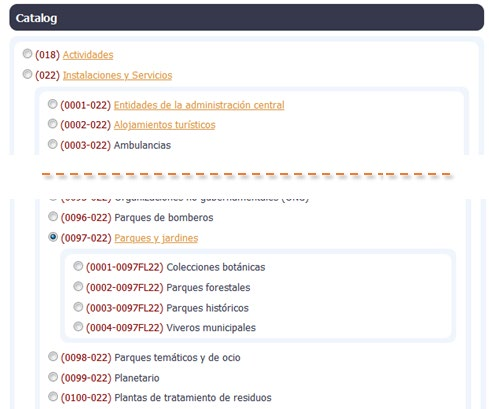
\includegraphics[width=\textwidth]{imagenes/Practica3fig1.jpg}
\caption{\label{fig:Practica3fig1.jpg}Representación de la estructura jerárquica de los concepts del catálogo de datos.}
\end{figure}


La aplicación por desarrollar recibirá como argumento el criterio de búsqueda, esto es, el código de la categoría de la que se desea información, y proporcionará información sobre los concepts y datasets pertinentes, aplicando para ello los siguientes criterios:

\begin{itemize}
    \item Se considerarán pertinentes el concept cuyo código (elemento code) coincida con el criterio de búsqueda y todos los concepts descendientes del mismo.
    \item Se considerarán pertinentes los dataset que contengan información asociada a alguno de los concept pertinentes (contengan un elemento concept con el atributo id igual al atributo id del elemento concept pertinente).
\end{itemize}

La Figura 2 muestra un ejemplo de búsqueda del concept con código 0097-022 y los resultados que se obtendrían.

\begin{figure}[H]
\centering
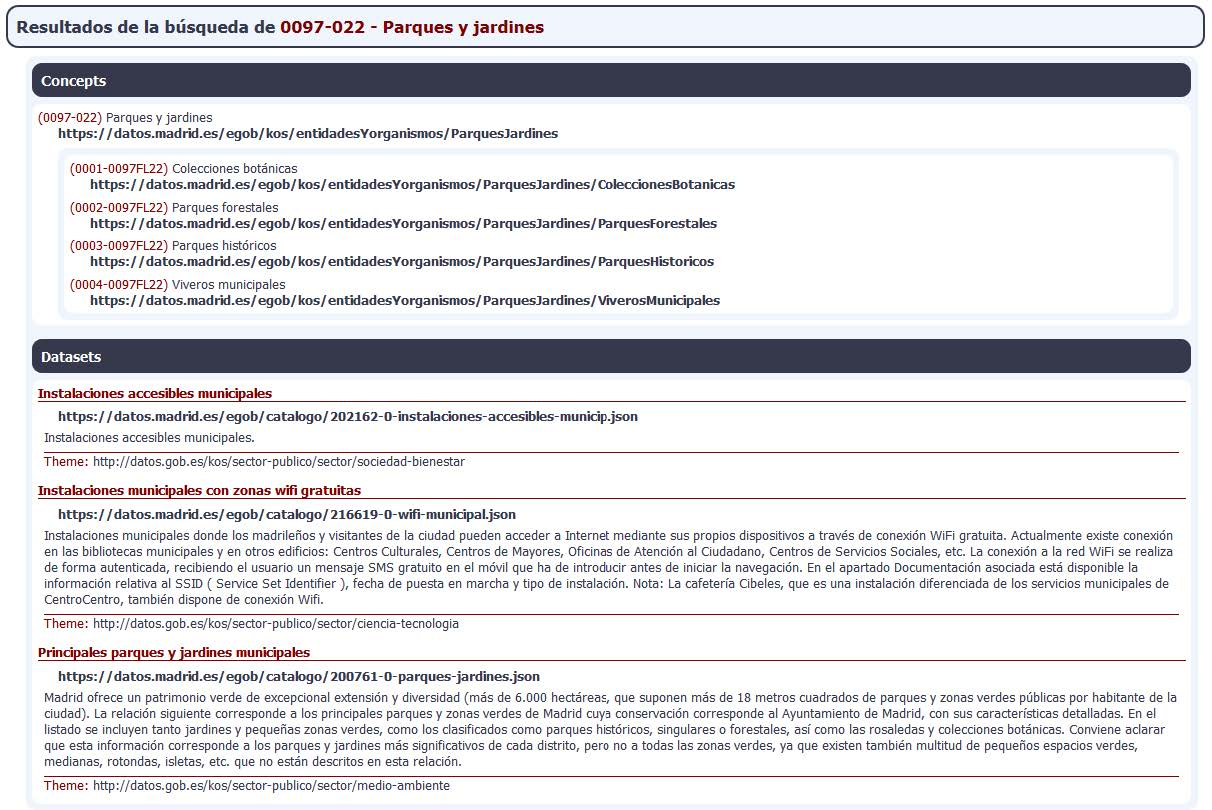
\includegraphics[width=\textwidth]{imagenes/Practica3fig2.jpg}
\caption{\label{fig:Practica3fig2.jpg}Concepts y datasets pertinentes para el código 0097-022.}
\end{figure}

\subsection{Desarrollo de la práctica}

La implementación de la Práctica 3 se basa en la creación de un analizador de documentos XML denominado XMLParser, desarrollado utilizando JavaCC, una herramienta que permite generar analizadores léxicos y sintácticos en el lenguaje Java. Este analizador se ha diseñado para procesar documentos XML que contienen datos publicados en el Portal de Datos Abiertos del Ayuntamiento de Madrid (http://datos.madrid.es).
Los documentos XML que se procesan a través de esta herramienta presentan ciertas características clave, como la identificación de recursos mediante URI, la asociación a categorías, la agrupación en conjuntos de datos y una clasificación jerárquica basada en características temáticas. La tarea principal del analizador es extraer información específica relacionada con códigos de categorías y, posteriormente, generar un nuevo documento XML que contiene los resultados deseados.

\subsection{Herramienta}
La principal herramienta desarrollada en esta práctica es el analizador XMLParser. Este analizador es capaz de llevar a cabo varias tareas esenciales:

\begin{itemize}
    \item Validación de argumentos de entrada para garantizar que los parámetros cumplan con las especificaciones requeridas.
    \item Extracción de información relevante de los documentos XML, siguiendo las reglas y estructuras definidas en la gramática.
    \item Generación de documentos de resultados que cumplen con un esquema específico.
\end{itemize}
El analizador XMLParser representa una contribución significativa en términos de procesamiento y manipulación de documentos XML.


\subsection{Conclusiones}

La Práctica 3 ha brindado a los estudiantes una experiencia valiosa en el manejo de tecnologías de análisis de documentos XML. A través del uso de JavaCC y la tecnología SAX, se ha proporcionado una base sólida para procesar información estructurada de manera eficiente. Los estudiantes han tenido la oportunidad de aplicar conceptos relacionados con la validación de argumentos, el análisis de elementos XML y la generación de documentos de resultados.
Uno de los aspectos más destacados de esta práctica es la capacidad de filtrar y seleccionar información relevante basada en códigos de categorías. Esta habilidad es fundamental en situaciones donde la extracción selectiva de datos es esencial.

\subsection{Preguntas Frecuentes}

¿Qué sentido tiene utilizar la clase ManejadorXML, si el parser ya busca lo que quiere?
Tiene sentido cronológico, ya que primero el parser realiza el análisis del documento y devuelve los datos, si se llama a una función que devuelva los datos es posible que se llamen a estas funciones antes de que se llame a la función de análisis

\subsection{Notas}

hacer clase concept con atributos code y label, hacer lista concepts de concept. hacer lo mismo con dataset. recoger los datos al igual que hacíamos en NXCalculator
Concepts, son objetos distintos, se tienen que reconocer de manera diferente. -> Nuevo objeto conceptInDataset
No hace falta un estado léxico, simplemente crear un objeto nuevo ya que son cosas diferentes, -> IncludedConcepts
String id -> idConcepts
XMLParser devuelve un objeto que tenga implementado la interfaz ParserCatalogo


\subsection{Código Fuente}

El código fuente de los archivos elaborados en esta practica se encuentra a continuación para su estudio y aprendizaje. Cabe destacar que se proporcionan dicho código para que el lector sea capaz de probar las funcionalidades con el objetivo de aprender mas acerca de las aplicaciones de JavaCC.

No se promueve el plagio y la realización de las prácticas, este simplemente es una de las muchas formas en las que se podría realizar la práctica.

\hyperref[sec:XMLParser]{XMLParser.jj}
%\href{https://shorturl.at/alqN6}{XMLParser.jj}

\section{Análisis de archivos JSON. Práctica 4}

\subsection{Introducción}

La Práctica 4 se centra en la exploración y aplicación de la tecnología GSON Streaming para el análisis y procesamiento eficiente de documentos JSON. El objetivo principal de esta etapa es familiarizar a los estudiantes con la API GSON Streaming y desarrollar un analizador de documentos JSON basado en esta tecnología. Como objetivo secundario, se busca capacitar a los estudiantes en el diseño de algoritmos eficientes para la extracción y transformación de información proveniente de fuentes de contenidos estructurados.

\subsection{GSON Streaming}

La API de transmisión de GSON es una API de Java que permite leer y escribir JSON de forma secuencial. Esto la hace útil en situaciones donde no es posible o deseable cargar el modelo de objeto completo en memoria, como cuando se trabaja con grandes cantidades de datos o cuando los datos se reciben de forma continua.

La API de transmisión de GSON se basa en dos clases principales: JsonReader y JsonWriter. JsonReader se utiliza para leer JSON de forma secuencial, mientras que JsonWriter se utiliza para escribir JSON de forma secuencial.

Las características principales de la API son su eficiencia en términos de memoria y  su flexibilidad. Por una parte, la API de transmisión de GSON no necesita cargar el modelo de objeto completo en memoria, lo que la hace más eficiente en términos de memoria que la API de GSON tradicional. Además, GSON Streaming permite leer y escribir datos JSON de forma secuencial, lo que la hace muy flexible.

La API es ideal para trabajar con grandes cantidades de datos, ya que puede leer y escribir los datos sin necesidad de cargarlos todos en memoria. También es ideal para recibir datos de forma continua, ya que puede leer los datos a medida que se reciben.


\subsection{JavaCC vs GSON Streaming}

\subsection{Descripción de la práctica}

La práctica busca ampliar la funcionalidad de la herramienta de búsqueda del Portal de Datos Abiertos del Ayuntamiento de Madrid, desarrollada en la Práctica 3. Se pretende dotar a esta herramienta de la capacidad para extraer información sobre los recursos asociados a una categoría específica (concept) del portal. Esto se logrará accediendo a los conjuntos de datos (dataset) en formato JSON y procesándolos con un analizador GSON Streaming.

El código desarrollado en la Práctica 3 servirá como punto de partida, y se completará para integrar un analizador GSON Streaming. Este analizador procesará la información de cada conjunto de datos pertinente y generará un documento XML válido conforme al esquema de documento ResultadosBusquedaP4.xsd. El nuevo elemento introducido en este esquema es resources, que contendrá información sobre los recursos asociados a las categorías pertinentes.

La generación del documento XML (indicado por ARG2) será similar al proceso de la Práctica 3, pero ahora se incorporará el elemento resources. Se utilizará la clase JSONDatasetParser para implementar el analizador GSON Streaming, y se analizarán los archivos .json indicados en el atributo id de cada dataset. Se añadirán como máximo cinco recursos (resource) a partir de cada dataset analizado.

\subsection{Desarrollo de la práctica}



\subsection{Herramienta}

La herramienta principal desarrollada en esta práctica es la extensión de la herramienta de búsqueda del Portal de Datos Abiertos, ahora mejorada con la capacidad de analizar y procesar datos JSON mediante la API GSON Streaming. La clase JSONDatasetParser representa la implementación de este analizador GSON Streaming. La herramienta final permite la extracción selectiva de información de archivos JSON, generando un documento XML conforme al esquema ResultadosBusquedaP4.xsd que incluye el nuevo elemento resources.

\subsection{Conclusiones}

La Práctica 4 ha proporcionado a los estudiantes una oportunidad única para aplicar sus conocimientos adquiridos en la Práctica 3 y explorar en profundidad la API GSON Streaming. La capacidad de extender la funcionalidad de la herramienta existente para manejar datos JSON y generar documentos XML enriquecidos demuestra una comprensión avanzada de las tecnologías de procesamiento de datos estructurados.

El uso de GSON Streaming versión 2.9.0 ha permitido a los estudiantes implementar un analizador eficiente para manejar grandes conjuntos de datos JSON, cumpliendo así con los requisitos de la práctica.

\subsection{Preguntas Frecuentes}

Pregunta 1: ¿Cuál es el propósito principal de la Práctica 4 en términos de procesamiento de información JSON?
Respuesta: El objetivo principal es extender la herramienta de búsqueda para extraer información sobre recursos asociados a categorías específicas en el Portal de Datos Abiertos, utilizando la tecnología GSON Streaming.

Pregunta 2: ¿Qué elemento se introduce en el esquema Resultados\\BusquedaP4.xsd ?
Respuesta: Se introduce el elemento resources, que contendrá información sobre los recursos asociados a las categorías pertinentes.

Pregunta 3: ¿Cuál es la versión de la API GSON Streaming utilizada en esta práctica?
Respuesta: Se utiliza la versión 2.9.0 de la API GSON Streaming, disponible en este enlace.

\subsection{Notas}

\subsection{Código Fuente}

El código fuente de los archivos elaborados en esta practica se encuentra a continuación para su estudio. Cabe destacar que se proporcionan dicho código para que el lector sea capaz de probar las funcionalidades con el objetivo de aprender mas acerca de las aplicaciones de JavaCC.

No se promueve el plagio y la realización de las prácticas, este simplemente es una de las muchas formas en las que se podría realizar la práctica.

\hyperref[sec:JSONParser]{JSONParser.jj}
%\href{https://shorturl.at/wFG45}{JSONParser.jj}

\section{Evolutivo de las prácticas}

\subsection{Introducción}

Como se ha podido observar de las prácticas de las secciones anteriores, pese a ser interesantes y cumplir con los objetivos establecidos de aprendizaje, son poco interesantes y se podría realizar unos ejercicios mas potentes y versátiles que exprimiesen al máximo las funcionalidades de las herramientas que hemos ido repasando.

Es por ello que en esta sección se plantea unos ejercicios a modo de evolutivo, que amplían los requerimientos y complejidad del análisis. Además se observará que, gracias al incremento en la complejidad de los ejercicios, aumenta en proporción la sencillez con la que se resuelven dichos problemas empleando JavaCC.

De esta forma, se podrá observar lo ventajoso de crear un analizador a la medida de usuario, y como JavaCC es una herramienta versátil y muy potente.

%La Práctica 5 representa una etapa crucial en el proyecto, enfocándose en la familiarización con la tecnología de transformación de documentos XML mediante el Lenguaje de Rutas de XML (XPath), basado en el Modelo de Objetos de Documento (DOM). El objetivo principal es extraer información del documento XML generado en la Práctica 4 utilizando expresiones XPath y almacenarla en un nuevo documento en formato JSON. Esta práctica permite a los estudiantes explorar técnicas avanzadas de manipulación de datos estructurados.

\subsection{Evolutivo 1. XML}

Este evolutivo se presenta a partir de la Practica 3. En dicha práctica se analizaban documentos xml, y se proponía analizar un documento xml con cierta recursividad

XPath, abreviatura de XML Path Language, es un lenguaje de consulta para documentos XML. Se utiliza para seleccionar partes de un documento XML, como elementos, atributos, texto y datos binarios.

XPath se basa en una sintaxis similar a la de las expresiones regulares. Las expresiones XPath se utilizan para construir caminos a través de un documento XML.

Las principales características de XPath son las siguientes:

    Selección de elementos: XPath se puede utilizar para seleccionar elementos individuales o conjuntos de elementos en un documento XML.
    Selección de atributos: XPath se puede utilizar para seleccionar atributos individuales o conjuntos de atributos de un elemento.
    Selección de texto: XPath se puede utilizar para seleccionar texto de un elemento o atributo.
    Selección de datos binarios: XPath se puede utilizar para seleccionar datos binarios de un elemento o atributo.


XPath se utiliza en una variedad de aplicaciones, incluyendo el procesamiento de XML, el desarrollo web, y la integración de datos. Esto permite que se utilize para procesar documentos XML, extraer datos, validar documentos y transformar documentos. Además, se utiliza en aplicaciones web para acceder a datos XML, como datos de formularios o datos de un servicio web. Por último, también se puede emplear para integrar datos de diferentes fuentes, como datos XML y datos de bases de datos.


\subsection{JavaCC vs XPath}

JavaCC y XPath son dos herramientas que se pueden utilizar para procesar documentos XML. Sin embargo, tienen algunas diferencias clave.

JavaCC es una herramienta de generación de analizadores sintácticos. Se utiliza para generar analizadores sintácticos que pueden analizar documentos XML.

Como ya hemos visto en secciones anteriores, las principales ventajas de JavaCC son su eficiencia en términos de memoria y su gran flexibilidad a los usuarios. Por otra parte, la principal desventaja de JavaCC es su dificultad de uso, 

XPath es un lenguaje de consulta para documentos XML. Se utiliza para seleccionar partes de un documento XML.

Las principales ventajas de XPath son su sencillez, ya que es una herramienta relativamente sencilla de aprender a utilizar, y su generalidad, pues se puede utilizar para procesar cualquier documento XML, independientemente de su lenguaje.

Las principales desventajas de XPath son su eficiencia, debido a que es menos eficiente en términos de memoria que JavaCC, y sus limitaciones, como la imposibilidad de procesar datos binarios.


\subsection{Descripción de la práctica}

La implementación de la Práctica 5 se basa en extender el código desarrollado en la Práctica 4, integrando la funcionalidad de XPath para extraer información específica del documento XML resultante. El uso del Modelo de Objetos de Documento (DOM) facilita la navegación y manipulación de la estructura jerárquica del documento XML.

Se requerirá la introducción de expresiones XPath para identificar y seleccionar los elementos deseados en el documento XML. La información obtenida mediante XPath se almacenará en un nuevo documento en formato JSON. Este proceso de transformación garantiza que la información relevante se extraiga eficientemente y se represente en un formato JSON para su posterior análisis o intercambio.

\subsection{Desarrollo de la práctica}

\subsection{Herramienta}

La herramienta principal desarrollada en esta práctica es una extensión del código existente en la Práctica 4, ahora mejorado con la capacidad de utilizar expresiones XPath para extraer información específica del documento XML resultante. La información extraída se guarda en un nuevo documento en formato JSON, ofreciendo una representación alternativa y flexible de los datos.

\subsection{Conclusiones}

La Práctica 5 proporciona a los estudiantes una valiosa experiencia en la utilización de XPath para la extracción selectiva de información de documentos XML. La capacidad de integrar esta tecnología con el código existente de la Práctica 4 demuestra la versatilidad en el manejo de datos estructurados.

El proceso de transformación a JSON destaca la flexibilidad de las tecnologías utilizadas, permitiendo la representación de datos en diferentes formatos según las necesidades del proyecto.

\subsection{Preguntas Frecuentes}

Pregunta 1: ¿Cuál es el propósito principal de la Práctica 5 en términos de transformación de datos?
Respuesta: El objetivo principal es la extracción de información específica del documento XML mediante expresiones XPath y la posterior representación de esta información en un nuevo documento en formato JSON.

Pregunta 2: ¿Cómo se realiza la transformación de datos de XML a JSON en esta práctica?
Respuesta: La transformación se realiza mediante la utilización de expresiones XPath para identificar y seleccionar información específica en el documento XML generado en la Práctica 4. La información seleccionada se almacena en un nuevo documento en formato JSON.

Pregunta 3: ¿Cómo se integra la funcionalidad XPath en el código existente de la Práctica 4?
Respuesta: Se realizarán modificaciones en el código de la Práctica 4 para incorporar expresiones XPath que seleccionen la información deseada. La información extraída se utilizará para generar un nuevo documento en formato JSON

\subsection{Notas}